\documentclass[tikz,border=10pt]{standalone}
\usepackage{tikz}
\usetikzlibrary{arrows.meta,positioning,fit,backgrounds,calc,shadows,shapes.geometric}

% Color definitions
\definecolor{lavenderDark}{RGB}{15, 44, 89}
\definecolor{lavenderDeep}{RGB}{10, 28, 58}
\definecolor{lavenderMedium}{RGB}{29, 78, 158}
\definecolor{lavenderLight}{RGB}{240, 246, 255}
\definecolor{lavenderBorder}{RGB}{180, 205, 237}
\definecolor{prismNavy}{RGB}{15, 44, 89}
\definecolor{prismBlue}{RGB}{29, 78, 158}
\definecolor{prismTeal}{RGB}{13, 148, 136}
\definecolor{prismMint}{RGB}{236, 253, 245}
\definecolor{prismGold}{RGB}{217, 119, 6}
\definecolor{prismDark}{RGB}{15, 23, 42}

\begin{document}
% Gantt Chart for SNN-Based Anomaly Detection and Tracking Project
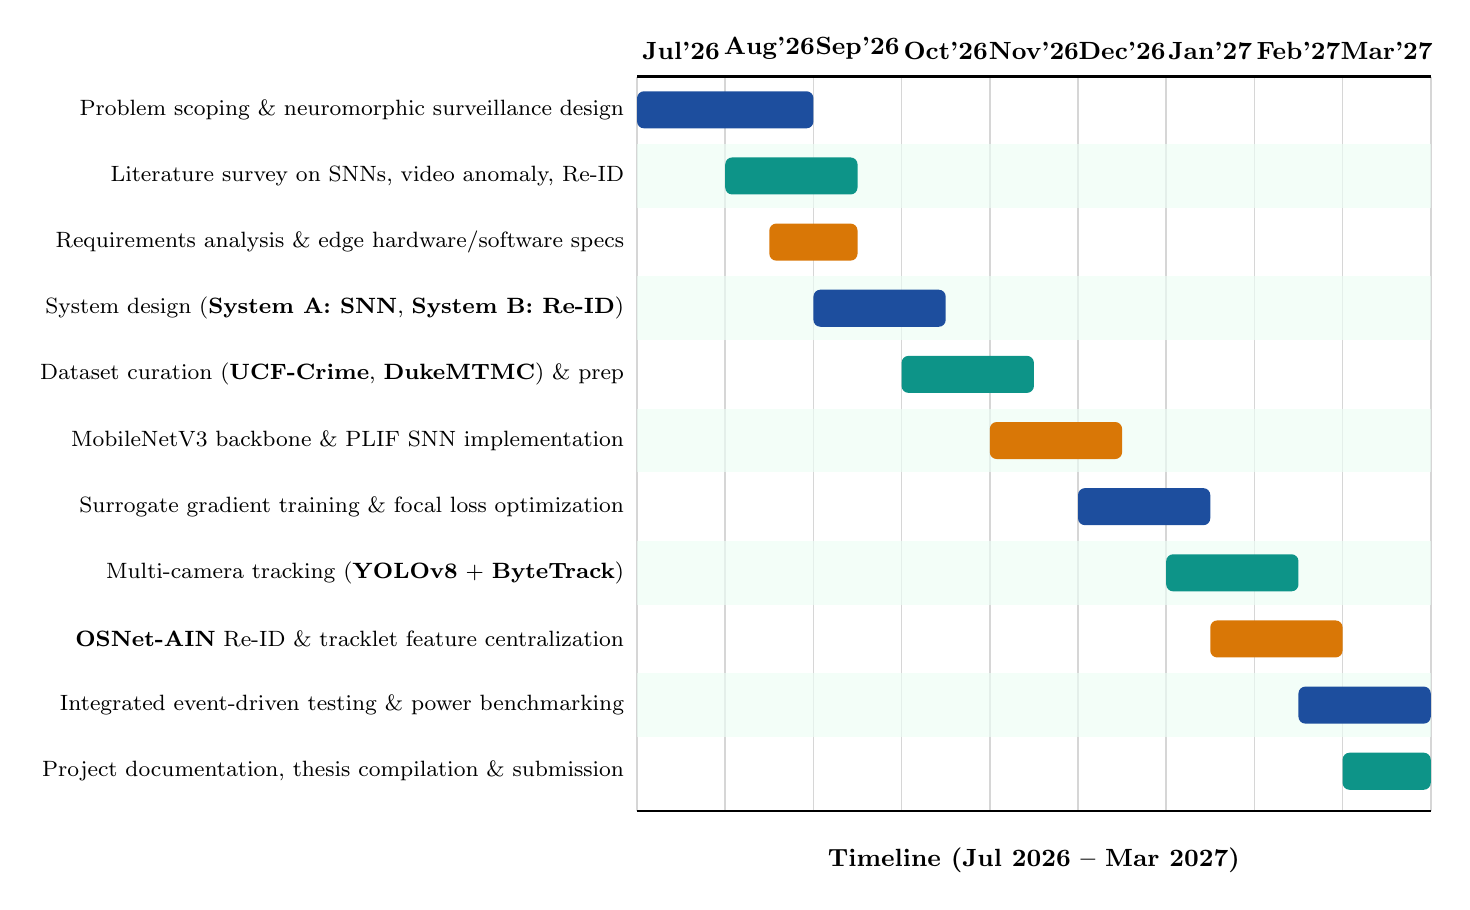
\begin{tikzpicture}[
  x=1.12cm, y=0.84cm,
  lab/.style={anchor=east, font=\fontsize{8.5}{10.5}\selectfont, inner sep=4.5pt, text=black}
]
\def\nm{9}
\def\topY{11.5}

% Vertical month gridlines
\foreach \i in {0,1,...,\nm} {
  \draw[gray!32, line width=0.55pt] (\i, 0.4) -- (\i, \topY);
}

% Month headers on top
\foreach \i/\m in {0.5/Jul'26, 1.5/Aug'26, 2.5/Sep'26, 3.5/Oct'26, 4.5/Nov'26, 5.5/Dec'26, 6.5/Jan'27, 7.5/Feb'27, 8.5/Mar'27} {
  \node[anchor=south, font=\fontsize{9.0}{11.0}\selectfont\bfseries, text=black] at (\i, \topY+0.12) {\m};
}
\draw[black, line width=1.0pt] (0, \topY) -- (\nm, \topY);
\draw[black, line width=0.8pt] (0, 0.4) -- (\nm, 0.4);

% Alternating row background shading
\foreach \k in {0,...,10} {
  \pgfmathsetmacro{\yc}{11.0-\k}
  \ifodd\k
    \fill[prismMint, opacity=0.65] (0, \yc-0.48) rectangle (\nm, \yc+0.48);
  \fi
}

% Task milestone labels on left
\node[lab] at (0, 11.0) {Problem scoping \& neuromorphic surveillance design};
\node[lab] at (0, 10.0) {Literature survey on SNNs, video anomaly, Re-ID};
\node[lab] at (0, 9.0)  {Requirements analysis \& edge hardware/software specs};
\node[lab] at (0, 8.0)  {System design (\textbf{System A: SNN}, \textbf{System B: Re-ID})};
\node[lab] at (0, 7.0)  {Dataset curation (\textbf{UCF-Crime}, \textbf{DukeMTMC}) \& prep};
\node[lab] at (0, 6.0)  {MobileNetV3 backbone \& PLIF SNN implementation};
\node[lab] at (0, 5.0)  {Surrogate gradient training \& focal loss optimization};
\node[lab] at (0, 4.0)  {Multi-camera tracking (\textbf{YOLOv8} + \textbf{ByteTrack})};
\node[lab] at (0, 3.0)  {\textbf{OSNet-AIN} Re-ID \& tracklet feature centralization};
\node[lab] at (0, 2.0)  {Integrated event-driven testing \& power benchmarking};
\node[lab] at (0, 1.0)  {Project documentation, thesis compilation \& submission};

% Milestone Gantt Bars
\fill[prismBlue, rounded corners=2.5pt]     (0.0, 11.0-0.28) rectangle (2.0, 11.0+0.28);
\fill[prismTeal, rounded corners=2.5pt]     (1.0, 10.0-0.28) rectangle (2.5, 10.0+0.28);
\fill[prismGold, rounded corners=2.5pt]     (1.5, 9.0-0.28)  rectangle (2.5, 9.0+0.28);
\fill[prismBlue, rounded corners=2.5pt]     (2.0, 8.0-0.28)  rectangle (3.5, 8.0+0.28);
\fill[prismTeal, rounded corners=2.5pt]     (3.0, 7.0-0.28)  rectangle (4.5, 7.0+0.28);
\fill[prismGold, rounded corners=2.5pt]     (4.0, 6.0-0.28)  rectangle (5.5, 6.0+0.28);
\fill[prismBlue, rounded corners=2.5pt]     (5.0, 5.0-0.28)  rectangle (6.5, 5.0+0.28);
\fill[prismTeal, rounded corners=2.5pt]     (6.0, 4.0-0.28)  rectangle (7.5, 4.0+0.28);
\fill[prismGold, rounded corners=2.5pt]     (6.5, 3.0-0.28)  rectangle (8.0, 3.0+0.28);
\fill[prismBlue, rounded corners=2.5pt]     (7.5, 2.0-0.28)  rectangle (9.0, 2.0+0.28);
\fill[prismTeal, rounded corners=2.5pt]     (8.0, 1.0-0.28)  rectangle (9.0, 1.0+0.28);

% Bottom title
\node[font=\fontsize{9.2}{11.2}\selectfont\bfseries, text=black] at (4.5, -0.35) {Timeline (Jul 2026 -- Mar 2027)};
\end{tikzpicture}
\end{document}
